\section{Sovereign Cloud Stack}
\label{sec:gaia-x:scs}

\begin{figure}[h]
  \centering
  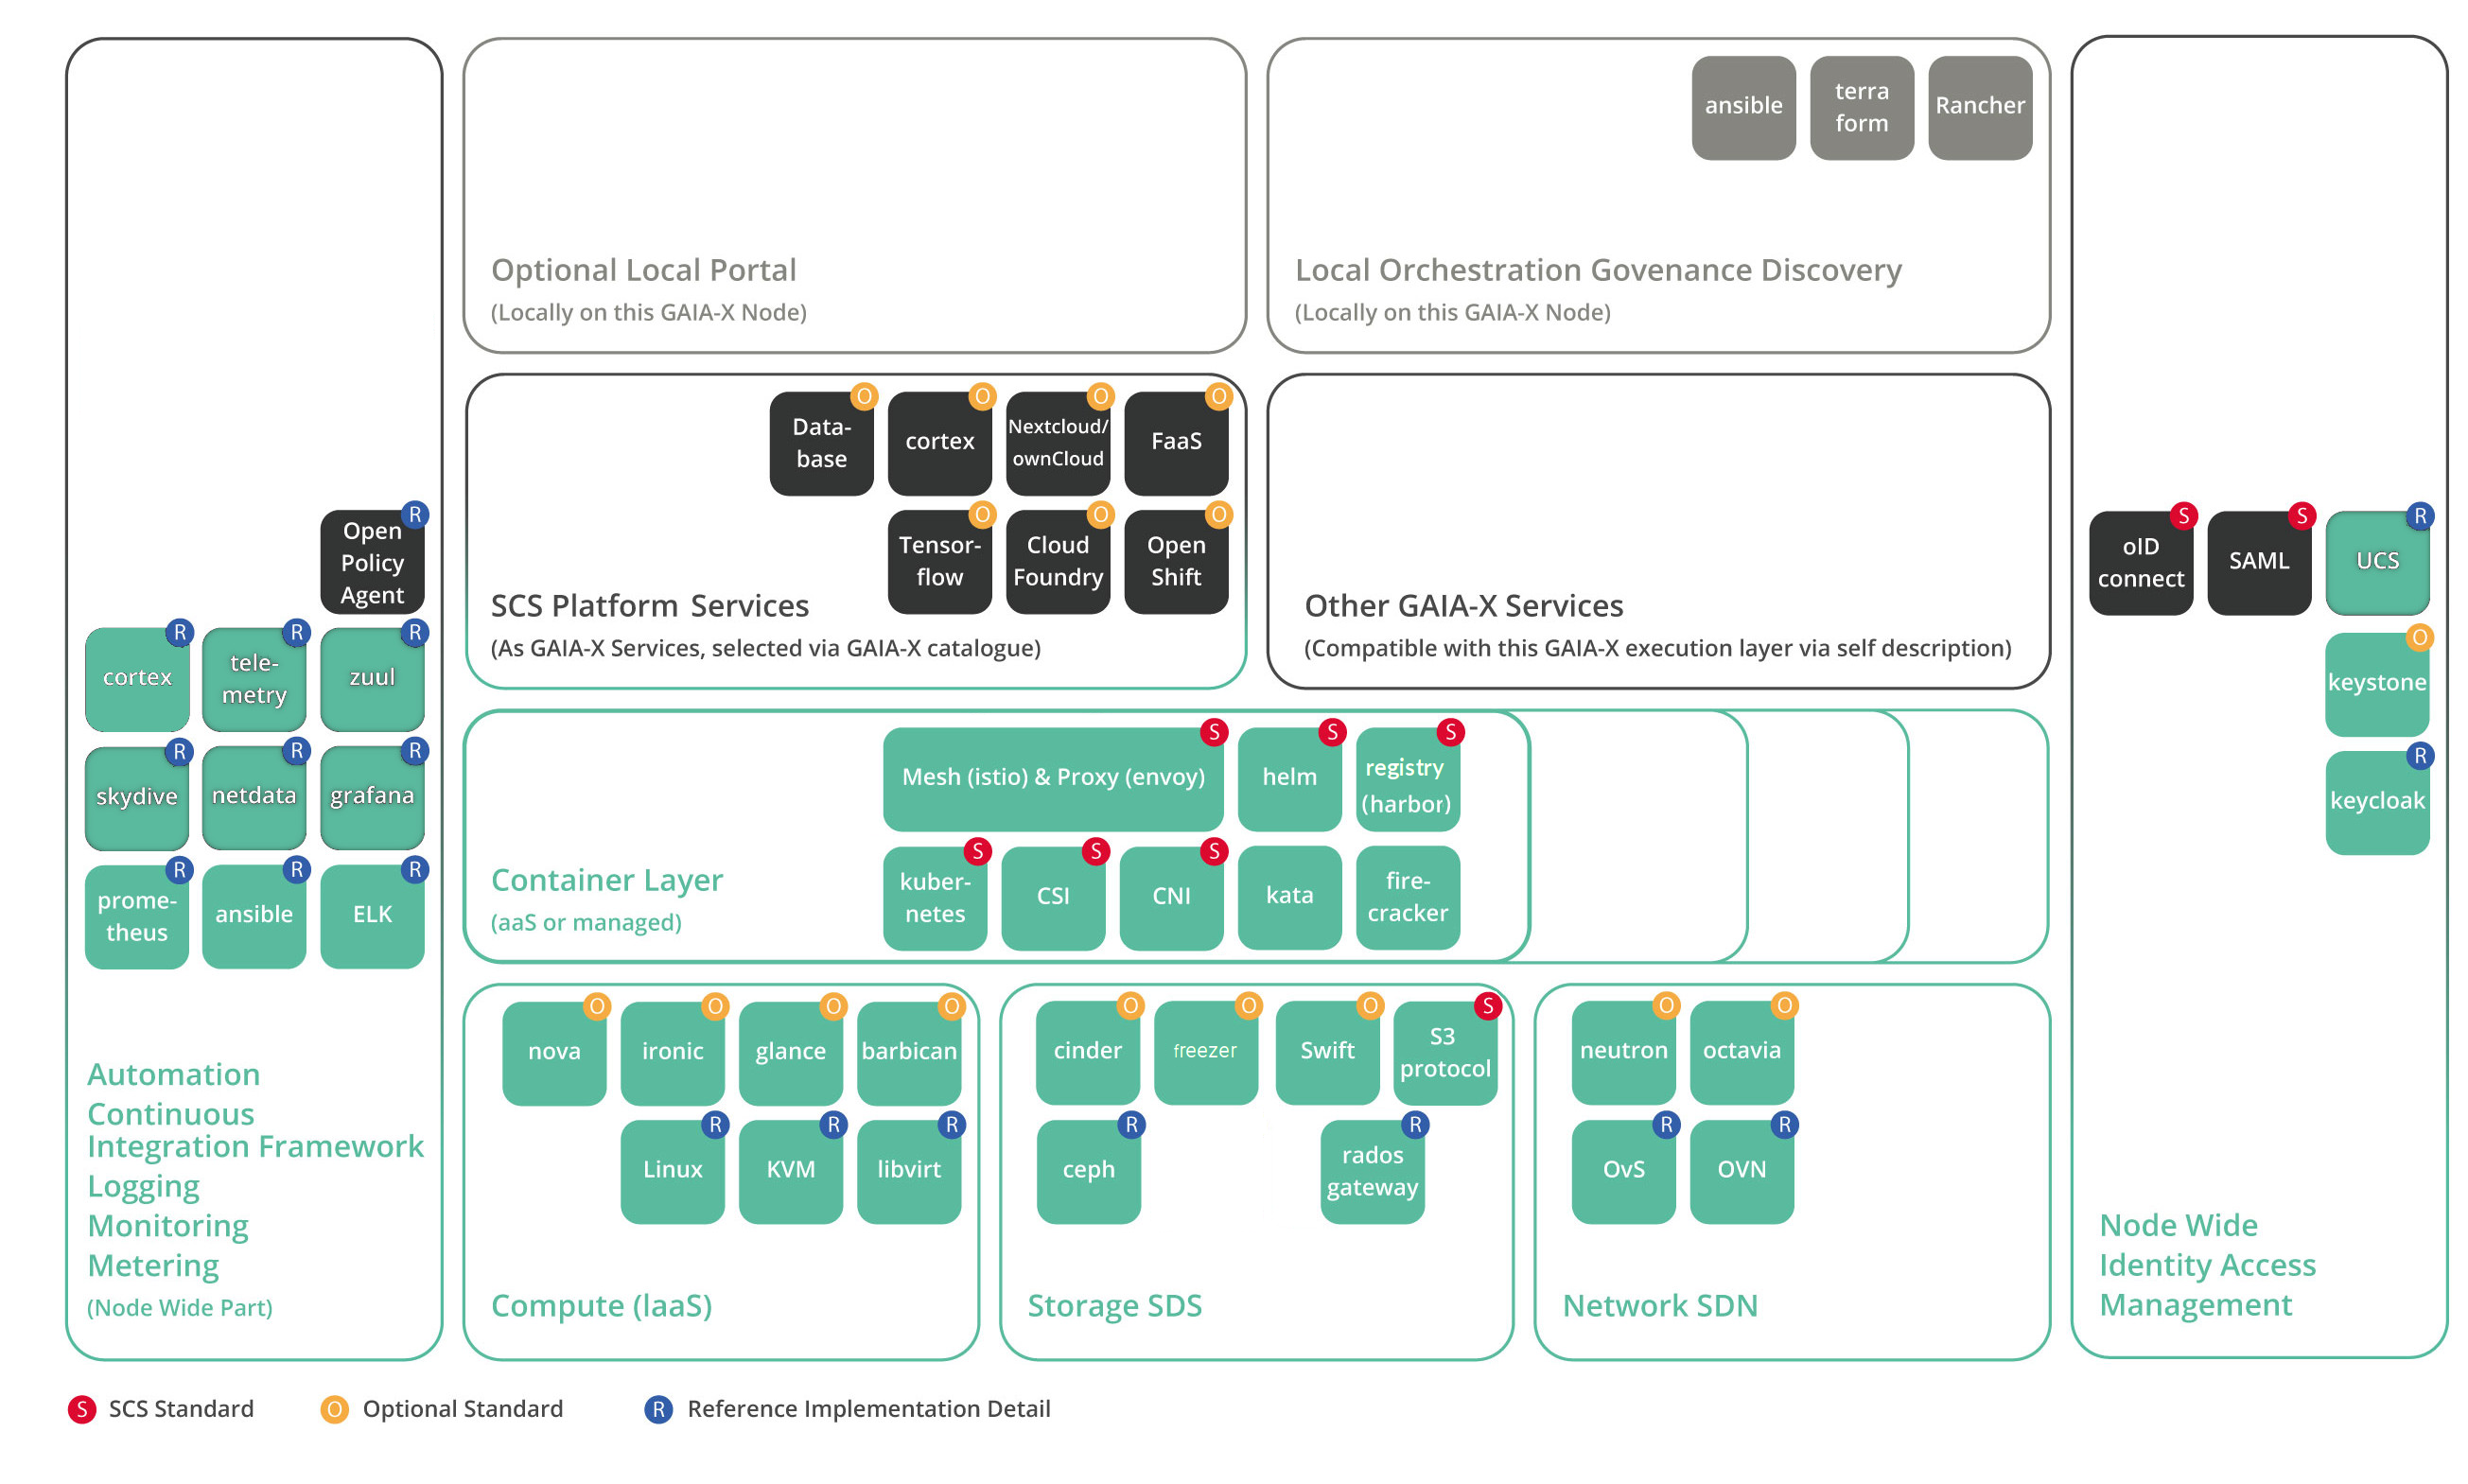
\includegraphics[height=0.71\textwidth]{gfx/chapters/4_gaia-X/scs_architecture.png}
  \caption{Architektur und Komponenten des Sovereign Cloud Stacks}
  \source{https://scs.community/assets/images/201001-SCS-4a.png}
  \label{fig:scs_architecture}
\end{figure}

\ac{SCS} ist ein Open-Source Projekt, um eine standartisierte und souveräne Plattform zu definieren, welche von 
existierenden und zukünfitgen Cloudprovidern genutzt werden soll. Hierbei soll der \ac{SCS} als Grundlage für Gaia-X Provider
dienen, um einen standartisiertes Umfeld zu schaffen.
Als technologischer Standpunkt dient \ref{fig:scs_architecture}, welches die geplante Architektur des \ac{SCS} zeigt. 
Grundlage des Stacks sind OpenStack Services, welche als OpenSource Projekt für Cloud-Computing Architektur entwickelt wurde.
Unterteilt wird dies in 3 grundlegende Bausteine: \textbf{Compute}, \textbf{Network} und \textbf{Storage}. Darauf aufbauend
wird ein Container Layer erstellt, welcher mit Hilfe von Docker oder Podman\footnote{\href{https://podman.io}{Podman}} gesteuert werden soll. \cite{scs}
Für die Entwicklung des Rocket Chat \ac{SaaS} wurde diese Architektur als Grundbild genutzt, indem 
genannte Technologien dieses Stacks in der Implementierung berücksichtigt wurden.